\documentclass[10pt,pdflatex,headrule,landscape]{beamer}
\setbeamertemplate{caption}[numbered]

\setbeamertemplate{bibliography item}[text]

\usepackage{psfrag}
\usepackage{graphics,wrapfig,lipsum}
\usepackage{subfig}
\usepackage{graphicx}
\usepackage{epsf}
\usepackage[english]{babel}
\usepackage{times}
\usepackage{amssymb}
\usepackage{amsmath}
\usepackage{amsfonts}
\mode<presentation> {
\usetheme{Warsaw}
\usecolortheme{seahorse}
\usecolortheme{rose}
\usefonttheme{professionalfonts}
}
\newcommand\vecnot[1]{\boldsymbol{#1}}
\newcommand\optvecnot[1]{\vecnot{#1}_{opt}}
\author{
Yehezkel Karo Itay\\[1cm]{Supervisor: Prof. Cohen Israel}\\{external supervisor: Dr. Dvorkind Tsvi}
}
\title{Feedback Based Spatial Beam-forming with Applications to Acoustic Signal Processing}

\institute[SFU]{
Department of Electrical Engineering \\
Technion - Israel Institute of Technology \\
Technion City, Haifa 3200003, Israel
}
\date[]

\newtheorem{property}{Property}[section]

\begin{document}

\begin{frame}
  \titlepage
\end{frame}

\begin{frame}
  \frametitle{Outline}
  \tableofcontents[hideallsubsections]
\end{frame}

\setlength{\parskip}{1em}

\section{Introduction}

\begin{frame}
\frametitle{Array processing}
Sensor array processing is a much studied subject.
\\
It has various implementations in multiple fields of research such as 
\begin{itemize}
 \item radar and sonar
 \item communication
 \item radio astronomy
 \item seismic science
 \item medical imaging and radiation
\end{itemize}
In particular, the uniform linear array (ULA), which consists of multiple equally spatially-spaced sensors (hence its name), is the basic, most studied array architecture.
\end{frame}

\begin{frame}
\frametitle{Spatial filtering}
One common array processing application is spatial filtering i.e. processing signals according to their spatial properties (direction-of-arrival - DOA) rather than their temporal properties (frequency).
\begin{itemize}
\item 
{
In receiver context, the array will enhance/attenuate signals according to their DOA, thus enabling better handling of interfering signals.
}
\item 
{
In transmitter context, the array will focus the transmitted signals to specific directions, thus enabling energy-efficient transmission.
}
\end{itemize}
\end{frame}

\begin{frame}
\frametitle{delay-and-sum beam-forming}
The most common basic beam-former is the delay-and-sum (Fig. \ref{fig:DelayAndSum}) which consists of weighted-and-summed ULA output signals which generates a spatially directed "beam" (Fig. \ref{fig:SimpleSpatialResponse}).
\begin{figure}%
    \centering
    \subfloat
    [Basic delay and sum architecture]
    {
    {
    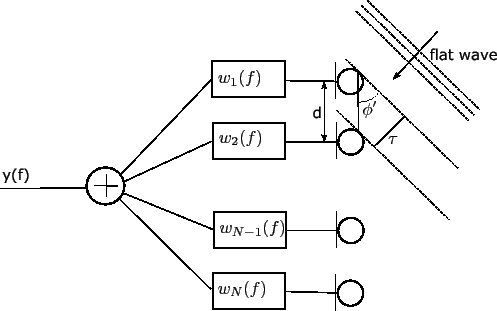
\includegraphics[width=0.35\textwidth]
    {Media/delay_and_sum_architecture.png}
    }
    \label{fig:DelayAndSum}
    }    
    \qquad
    \subfloat
    [Basic spatial response]
    {
    {
    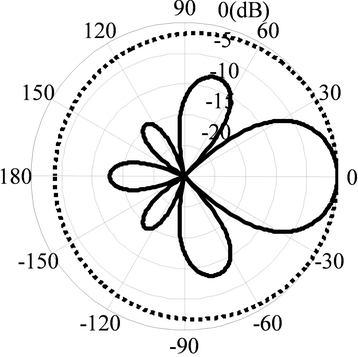
\includegraphics
    [width=0.2\textwidth]
    {Media/simple_spatial_response.PNG}
    }
    \label{fig:SimpleSpatialResponse}
    }
    \caption{Delay-and-sum filter and its spatial response.}
    \label{fig:delayAndSumArchAndResponse}    
\end{figure}
\end{frame}

\begin{frame}
\frametitle{signal processing fundamentals - filters}
\begin{itemize}
\item{
From signal processing theory, the most basic element would be the filter.
}
\item{
A filter is a linear system, consists of delay, gain and sum elements. For each filter, according to its demanded response, one can quantify the number of elements that should be used in the implementation, i.e. resource usage.
}
\item{
Filters are designed to enhance/attenuate/extract signals with specific features from a given signal.  
}
\item{
A filter can be described by its impulse response. i.e. the filter's expected output when the input signal is a single impulse.  
}
\item{
Each filter generates a specific response with respect to the relevant signal features of interest which can be mathematically derived from its impulse response.
}
\item{
In temporal domain, the signal feature of interest it is the frequency where in the spatial domain, it is the DOA.
}
\end{itemize}
\end{frame}

\begin{frame}
\frametitle{FIR vs. IIR}
\begin{minipage}{0.65\textwidth}
Filters can be divided to two main groups. 
\begin{itemize}
\item{
\textbf{Finite impulse response - FIR}
\\
Features configurable linear phase response which basically means that each frequency travels the filter in the same amount of time (no dispersion).
}
\item{
\textbf{Infinite impulse response - IIR}
\\
Although suffering dispersion, IIR filters are very efficient in terms of resource usage, featuring "sharper" gain responses with less resources.
}
\end{itemize}
\end{minipage}
\begin{minipage}{0.34\textwidth}
\begin{figure}
\captionsetup{font={scriptsize},labelfont={scriptsize}}
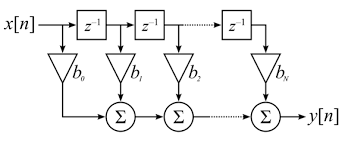
\includegraphics[width=0.9\textwidth]{Media/BASIC_FIR_FILTER_ARCH.png}
\caption{Basic FIR filter architecture - simple delay, weight \& sum.}
\end{figure}
\begin{figure}
\captionsetup{font={scriptsize},labelfont={scriptsize}}
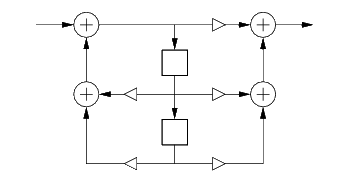
\includegraphics[width=0.8\textwidth]{Media/BASIC_IIR_FILTER_ARCH.png}
\caption{Basic IIR filter architecture - feedback based delay, weight \& sum.}
\end{figure}
\end{minipage}
\end{frame}

\begin{frame}
\frametitle{ULA as a spatial FIR}
\begin{minipage}{0.55\textwidth}
The similarity between a ULA (of distance $ d $ between consecutive elements) which receives a single impinging wavefront of DOA $ \theta $ to a FIR filter with sampling interval of $ \tau_{\theta}=\frac{d\cos{\theta}}{c} $ (where $ c $ is the signal propagation velocity) is obvious and well studied \cite{van1988beamforming}.
\end{minipage}
\begin{minipage}{0.44\textwidth}
\begin{figure}
\captionsetup{font={scriptsize},labelfont={scriptsize}}
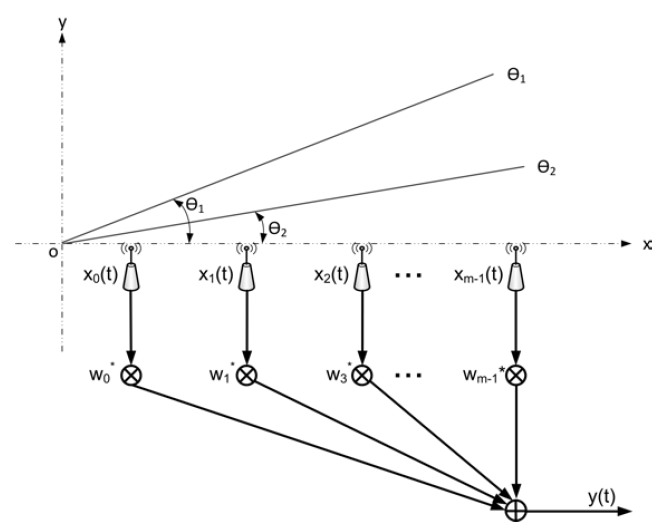
\includegraphics[width=\textwidth]{Media/ULA_FIR_similarity.PNG}
\caption{ULA and FIR similarity}
\end{figure}
\end{minipage}
\end{frame}

\section{Research goal}

\begin{frame}
\frametitle{Research main goal - Spatial \textbf{IIR}?}
The fundamental question driving this research is \\
\textbf{
``what is the array structure in spatial domain which is analogous to IIR filtering in the time domain?''
}
\\
which was already presented (but not fully answered) by Wen in his PhD thesis \cite{wen2013array}.
\label{frm:ResearchMainGoal_SpatialIIR}
\end{frame}

\begin{frame}
\frametitle{Previously proposed methods for achieving ``Spatial-IIR'' - 1/3}
In Wen's \cite{wen2013array} work and other works also \cite{Madanayake2008ABeamformer,Madanayake2009SystolicWDFs,Madanayake2008AFilters,Bruton2003Three-dimensionalBanks,Ward1986ABeamforming,Joshi2012SynthesisApplications}, some interesting methods were proposed for achieving ``Spatial-IIR'' but none of them truly achieved the IIR response solely in the spatial (i.e. $ \theta $) domain.
\\
\begin{minipage}{0.75\textwidth}
\begin{itemize}
\item
{
Wen's first method was to estimate $ \theta $ and approximate $ \tau_{\theta} $ accordingly for the feedback part of the IIR. 
\\
This method constrains the system to single speaker scenario and is suspected of high sensitivity to DOA estimation errors.
}
\end{itemize}
\end{minipage}
\begin{minipage}{0.24\textwidth}
\begin{figure}
\captionsetup{font={scriptsize},labelfont={scriptsize}}
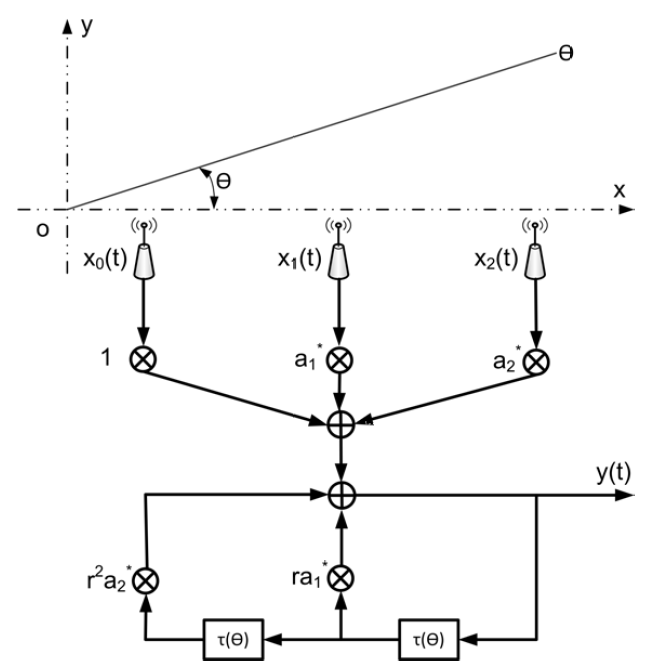
\includegraphics[width=\textwidth]{Media/WenFirstSuggestedMethod.PNG}
\caption{Wen's first suggested method - DOA estimation and approximated synthetic feedback delay.}
\end{figure}
\end{minipage}
\end{frame}

\begin{frame}
\frametitle{Previously proposed methods for achieving ``Spatial-IIR'' - 2/3}
\begin{minipage}{0.75\textwidth}
\begin{itemize}
\item
{
Wen's second method was to use shifted sub arrays (see Fig.\ref{fig:ShiftedSubArraysWen}) of the original array, thus obtaining $ \tau_{\theta} $ temporal separation between consecutive sub arrays output just as in IIR filter.
\\
Close examination unveils the fact that it is practically a complicated way for creating FIR response.
}
\end{itemize}
\end{minipage}
\begin{minipage}{0.24\textwidth}
\begin{figure}
\captionsetup{font={scriptsize},labelfont={scriptsize}}
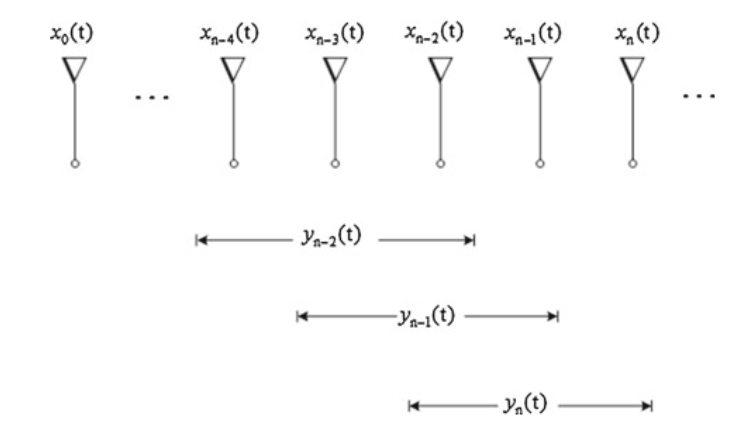
\includegraphics[width=\textwidth]{Media/SpatialIIR_SubArrays.PNG}
\caption{Shifted sub arrays to emulate IIR filter}
\label{fig:ShiftedSubArraysWen}
\end{figure}
\end{minipage}
\end{frame}

\begin{frame}
\frametitle{Previously proposed methods for achieving ``Spatial-IIR'' - 3/3}
\begin{minipage}{0.75\textwidth}
\begin{itemize}
\item
{
The other mentioned works use 2-D spatio-temporal filtering. In particular, the wavefront is viewed as a two dimensional signal, and the processing is done by performing IIR filtering in the time domain, but only FIR filtering (using a finite number of sensors) is performed in the spatial domain.
As can be seen in Fig.\ref{fig:SpatioTemporalPlaneWavePracticalFilter} taken from \cite{Bruton2003Three-dimensionalBanks}, the obtained 2-D filter is not ideal, causing imperfections in the overall spatial response.
}
\end{itemize}
\end{minipage}
\begin{minipage}{0.18\textwidth}
\begin{figure}
\captionsetup{font={scriptsize},labelfont={scriptsize}}
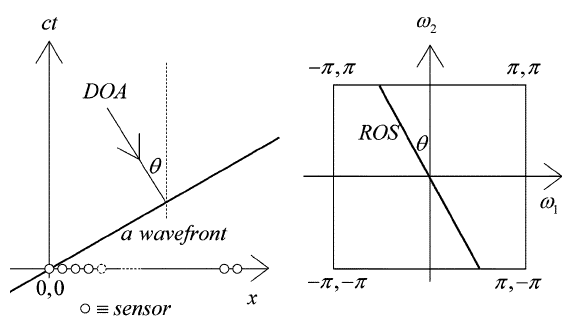
\includegraphics[width=\textwidth]{Media/SpatioTemporalPlaneWave.PNG}
\caption{Spatio-temporal representation of plane wave}
\label{fig:SpatioTemporalPlaneWave}
\end{figure}
\begin{figure}
\captionsetup{font={scriptsize},labelfont={scriptsize}}
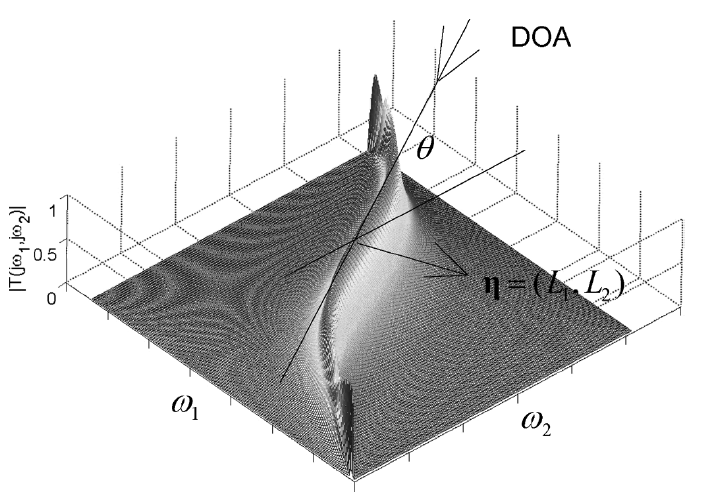
\includegraphics[width=\textwidth]{Media/SpatioTemporalPlaneWavePracticalFilter.PNG}
\caption{Practical spatio-temporal 2D plane-wave filter.}
\label{fig:SpatioTemporalPlaneWavePracticalFilter}
\end{figure}
\end{minipage}
\end{frame}

\section{Signal Model and Problem Formulation}

\begin{frame}
\frametitle{Signal Model - suggested system architecture}
\begin{minipage}{0.55\textwidth}
To fully answer the question presented in frame \ref{frm:ResearchMainGoal_SpatialIIR}, we proposed the following feedback-based system design (see Fig. \ref{fig:SpatialIIRSuggestedArch}) which, as will be shown, yields an IIR response with respect to $ \theta $, hence achieving the desired ``Spatial-IIR''.
\\
\\
\\
As can be seen, the cooperative speaker will hold a transponder which will transmit, in addition to the speaker's own signal, a synthetic signal which will be fed back to him. 
\end{minipage}
\begin{minipage}{0.44\textwidth}
\begin{figure}
\captionsetup{font={scriptsize},labelfont={scriptsize}}
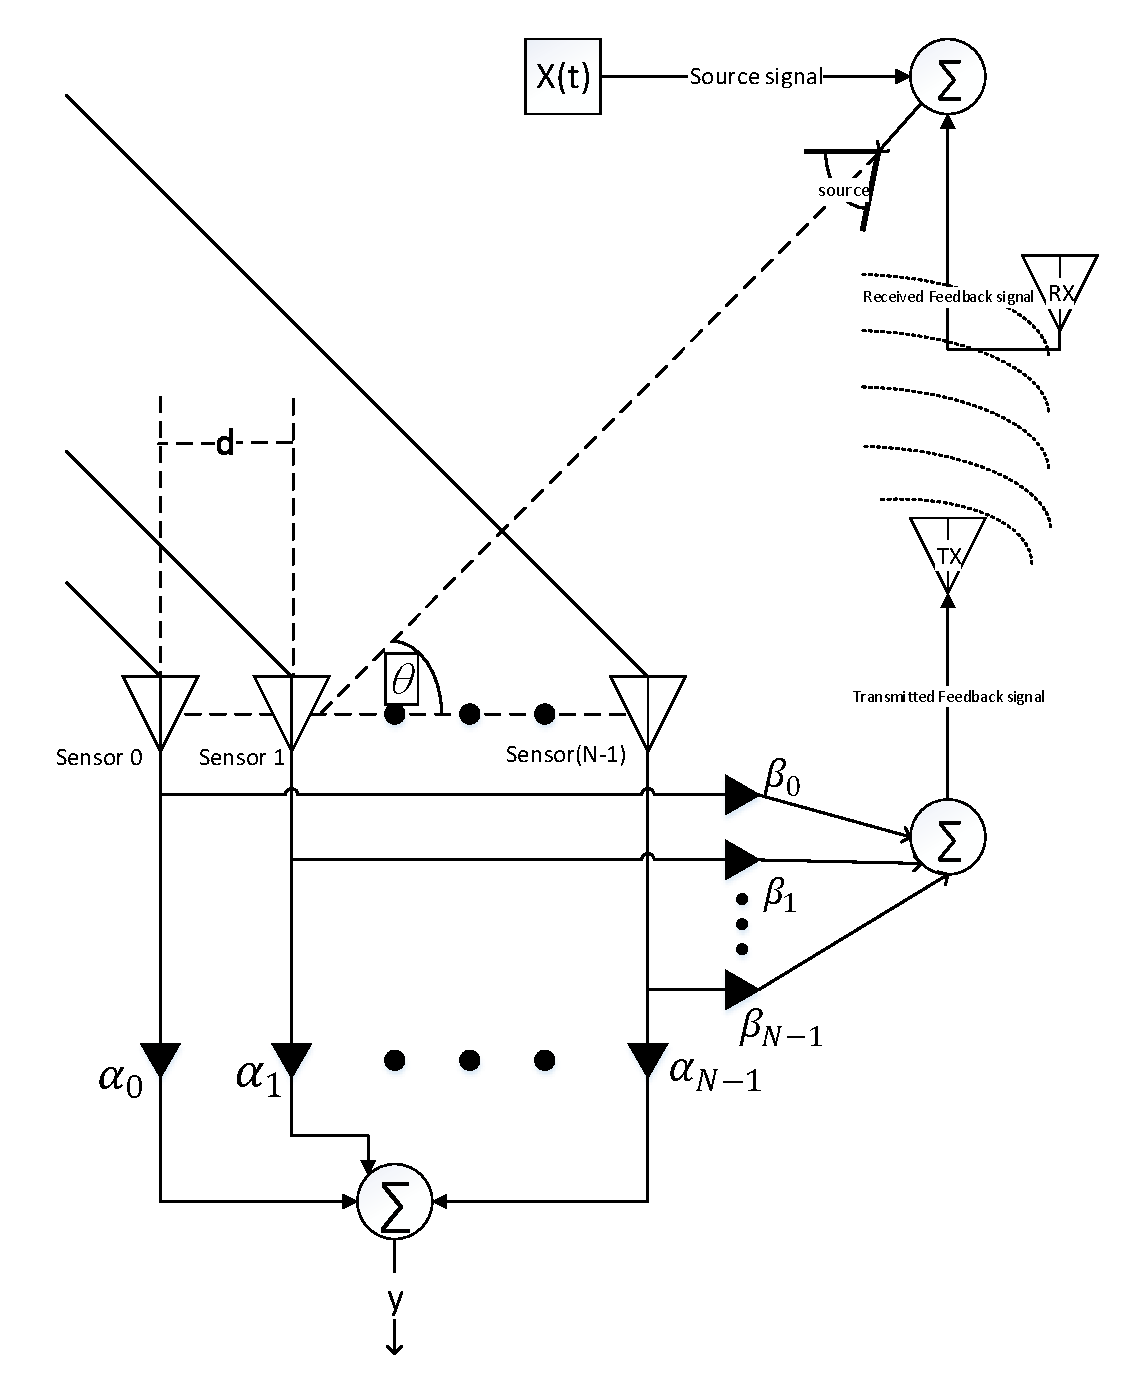
\includegraphics[width=\textwidth]{./Media/SpatialIIR-diagram/SpatialIIR_VER4.pdf}
\caption{Proposed system feedback-based architecture}
\label{fig:SpatialIIRSuggestedArch}
\end{figure}
\end{minipage}
\end{frame}

\begin{frame}[allowframebreaks]
\frametitle{Resolving the system transfer function}
Denoting:\\
$ x $ - source signal,\\
$ y $ - beamformer output,\\
$ \vecnot{\alpha},\vecnot{\beta} $ - user-controlled coefficient vectors,\\
$\vecnot{d}_{\theta}$ - steering vector with n'th element $e^{-j\omega \tau_{n,\theta}}$,\\
$ \tau_{pd} $ - propagation delay from the source to the reference sensor,\\
$ \tau_{tx} $ - feedback transmission delay\\
and assuming a simple flat channel, the equation which defines the \textbf{received signal at the n'th sensor}, and due to a wavefront from DOA $\theta$ is 
$$
x_{n,\theta}(t) = x(t-\tau_{pd}-\tau_{n,\theta})+\sum_{m=0}^{N-1}{\beta_{m}x_{m,\theta}(t-\tau_{pd}-\tau_{tx}-\tau_{n,\theta})}
$$
which, after taking all the array elements into account converts to
$$
\ifdefined\DEFIncludeAttenuation
    y^{\mathcal{F}}_{\theta}(\omega) 
    = 
    \vecnot{\alpha}^{T}
    \left(
    I
    -g^{2}\vecnot{d}_{\theta}
    \vecnot{\beta}^{T}
    e^{-j\omega(\tau_{pd}+\tau_{tx})}
    \right)
    ^{-1}
    g^{2}
    \vecnot{d}_{\theta}
    x^{\mathcal{F}}(\omega)
    e^{-j\omega\tau_{pd}}
\else
    y^{\mathcal{F}}_{\theta}(\omega) 
    = 
    \vecnot{\alpha}^{T}
    \left(
    I
    -\vecnot{d}_{\theta}
    \vecnot{\beta}^{T}
    e^{-j\omega(\tau_{pd}+\tau_{tx})}
    \right)
    ^{-1}
    \vecnot{d}_{\theta}
    x^{\mathcal{F}}(\omega)
    e^{-j\omega\tau_{pd}}
\fi
$$
under the Fourier transform.
\\
Using the Woodbury matrix identity \cite{woodbury1950inverting} yields
$$
\ensuremath{
y_{\theta}^{\mathcal{F}}(\omega) 
=
\frac
{
\vecnot{\alpha}^{T}
\vecnot{d}_{\theta}
exp\left(-j\tau\right)
}
{
1
-
\vecnot{\beta}^{T}\vecnot{d}_{\theta}
exp\left(-j\tau\right)
}
x^{\mathcal{F}}(\omega)
}
$$

\end{frame}

\section{Research tasks \& hurdles}

\begin{frame}
\frametitle{Future tasks}
For fully answering the question presented in frame \ref{frm:ResearchMainGoal_SpatialIIR}, we will 
\begin{itemize}
\item
{
Develop a method for choosing the optimal coefficients for $ \vecnot{\alpha},\vecnot{\beta} $.
}
\item
{
Study the system's stability properties.
}
\item
{
Implement a real world demo.
}
\end{itemize}
\end{frame}

\begin{frame}
\frametitle{Known issues and intended methods for resolving them}
After some initial simulations we can mark some of the issues that should be resolved and also provide suggestion for solving them.
\begin{itemize}
\item
{
\textbf{Stability under partial knowledge of $ \tau_{pd} $ and $ \tau_{tx} $}
\\
We found a very significant sensitivity to errors in partial knowledge scenarios which constrain us to know the range of the speaker with an unreasonable accuracy.
\\
To overcome this issue, we searched for works on low-sensitivity IIR filter design, baring in mind that \textbf{input errors may be treated as coefficient errors}, and came across the works of Stoyanov \cite{I.P.Topalov1990LOW-SENSITIVITYCYCLES,StoyanovNEWSECTIONS}, which suggest the following scheme:
\begin{itemize}
\item{Factorization of a given IIR to multiple $ 2^{nd} $ order sections}
\item{Modifying each section to have low sensitivity to coefficients error}
\item{Re-synthesizing the IIR from the ``immunized'' sections}
\end{itemize}
}
\end{itemize}
\end{frame}

\section{Conclusion}

\begin{frame}
\frametitle{Conclusion}
We believe that the suggested method, although yet fully stabilized, achieves the longed-for spatial-only IIR-like response and could hopefully serve as a fertile ground for future research and new interesting architectures or new feedback based systems implementations. 
\\
It can be implemented in additional scenarios such as 
\begin{itemize}
\item{Electro-magnetic environment - Radar \& communication}
\item{Different mediums - such as under-water acoustics}
\end{itemize}
and more.
\end{frame}


\begin{frame}[allowframebreaks]
\frametitle{References}
\bibliographystyle{unsrt}
\tiny{\bibliography{./Modules/Mendeley,./Modules/LocalBib}}
\end{frame}

\end{document}
